\documentclass[11pt,dvipdfmx,cjk]{beamer}
% パッケージの追加
\usepackage{graphicx} % 図を表示するためのパッケージの追加
\usepackage{bm} % 太字イタリックを使えるようにする 
\usepackage[labelformat=empty]{caption}
\usepackage{multirow}

% beamer に関する設定
% Adobe Reader の文字化けを防ぐおまじない
\AtBeginDvi{\special{pdf:tounicode EUC-UCS2}}
%テーマの指定
\usetheme{Singapore}
\renewcommand{\kanjifamilydefault}{\gtdefault} % 日本語をゴシック体にする
%\mathversion{bold} % これを指定するとデフォルトの数式が太字になる
%\usefonttheme{structurebold}

%--- colorblock 環境の定義
\setbeamercolor{upcolor}{fg=black,bg=blue!40} % ヘッダー部の色指定
\setbeamercolor{lowcolor}{fg=black,bg=blue!20} % body部の色指定
\setbeamertemplate{navigation symbols}{} % 右下に出てくるナビゲーションシンボルを消し飛ばす
\newenvironment{colorblock}%
{\begin{beamerboxesrounded}[upper=upcolor,lower=lowcolor,shadow=true]}%
{\end{beamerboxesrounded}}%
\usefonttheme{professionalfonts}
%itemizeの設定
%\setbeamertemplate{itemize item}{\normalsize\raise1.0pt\hbox{$\bullet$}}
%\setbeamertemplate{itemize subitem}{\normalsize\raise1.0pt\hbox{$\blacktriangleright$}}
%\setbeamertemplate{itemize subsubitem}{\normalsize\raise1.0pt\hbox{$\bigstar$}}
\setbeamertemplate{itemize item}{\normalsize\raise0.5pt\hbox{$\bullet$}}
\setbeamertemplate{itemize subitem}{\normalsize\raise1.0pt\hbox{$\blacktriangleright$}}
\setbeamertemplate{itemize subsubitem}{\normalsize\raise1.5pt\hbox{$\bigstar$}}
\renewcommand{\baselinestretch}{1.1}  % 行間設定

% 本文のタイトルなど
\title{Artificial Bee Colonyアルゴリズムによる\\サポートベクターマシン
のハイパーパラメータ最適化}
\author{2131007 安達 拓真}
\institute{千葉工業大学 情報科学部 情報工学科 4年 山口研究室}
\date{2024年1月24日}


\begin{document} % ここから本文

% タイトルページ表示
\begin{frame}
\maketitle
\end{frame}

\section{はじめに}

\begin{frame}
  \frametitle{はじめに}
  \begin{itemize}
    \item 機械学習にとってハイパーパラメータはモデルの性能を\\決める重要な値
    \item ハイパーパラメータを自動で調整する研究が行われている
    \item 先行研究として,Artificial Bee Colony(ABC)アルゴリズムを用いて,
    サポートベクターマシン(SVM)のハイパーパラメータ最適化と特徴選択を行った研究がある
    \item 本研究では,先行研究で最適化対象ではなかったカーネル関数をハイパーパラメータとして扱う手法を提案する
  \end{itemize}
\end{frame}
\section{既存手法} % セクションを入れると PDF に反映される
\begin{frame}
\frametitle{サポートベクターマシン(SVM)}
\begin{itemize}
    \item 1995年に提案された,分類や回帰に使用される機械学習\\アルゴリズム\footnote{ Cortes, C. and Vapnik, V. Support-vector networks, Ma-chine Learning, Vol.20, No.3, pp.273-297, 1995.}
    \item 非線形データを高次元空間に写像し,線形分離可能にする 
    \item データを分類する最適な境界線(超平面)を探す                
  \end{itemize}
  \begin{figure}
    \centering
    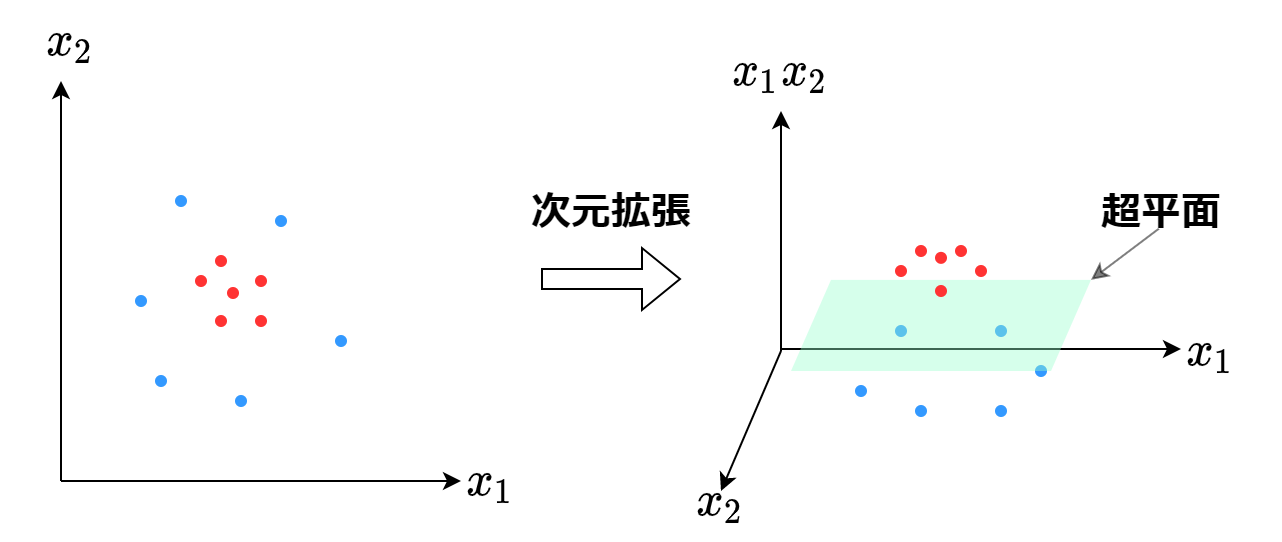
\includegraphics[width=0.8\linewidth]{syazou.png}
   \end{figure}
\end{frame}


%   \frametitle{ハイパーパラメータ最適化(HPO)}
 %   \begin{itemize}
  %    \item 機械学習の性能を最大限に発揮するには適切な\\ハイパーパラメータの設定が必要不可欠
  %    \item 手動では経験的に決めることが多く時間のかかる作業
  %     \begin{itemize}
  %       \item 自動で調節する研究が行われている
   %    \end{itemize}
   %   \item 一般的に計算量が大きいため効率的な探索が必要
   %   \item 離散値、連続値、カテゴリ変数など様々な値を扱う必要がある
   % \end{itemize}
  %\end{frame}
  \begin{frame}
    \frametitle{Artificial Bee Colony(ABC)アルゴリズム}
    \begin{itemize}
      \item 蜂の採餌行動に着目した最適化アルゴリズム\footnote{Karaboga, Dervis. An idea based on honey bee swarm for numerical optimization. Vol. 200. Technical report-tr06, Erciyes university, engineering faculty, computer engineering department, 2005.}
      \item 働き蜂,追従蜂,偵察蜂の三種類の蜂によって各食物源の\\探索を行い,最適解を求める
      \item 最適化対象は実数値
      \item ABC自体の設定パラメータは少ない
    \end{itemize}
  \end{frame}


  \begin{frame}
    \frametitle{先行研究\footnote{近藤 久,浅沼 由馬“人工蜂コロニーアルゴリズムによるランダムフォレストとサポートベクトルマシン
    のハイパーパラメータ最適化と特徴選択”,人工知能学会論文誌, vol34-2, pp.1-11, 2019.}におけるSVMのハイパーパラメータ最適化}
    \begin{itemize}
      \item カーネル関数をRBFカーネルに固定
      \item  最適化にはABCを使用
      \item 最適化したハイパーパラメータ
      \begin{itemize}
        \item SVMの$C$
        \item RBFカーネルの$\gamma$
      \end{itemize}
      %式書いたほうがいいかも
    \end{itemize}
\end{frame}

\section{提案手法}
  \begin{frame}
    \frametitle{問題点}
    \begin{itemize}
      \item カーネル関数をRBFカーネルに固定している
      \begin{itemize}
       \item SVMにはRBFカーネル以外にも様々なカーネル関数が適用できる      
      \item カーネル関数によってハイパーパラメータが異なる
    \end{itemize}
    \item ハイパーパラメータ空間の探索範囲が限定的
  \end{itemize}
\end{frame}
  
  \begin{frame}
    \frametitle{提案手法}
    \begin{itemize}
      \item 以下の4つのカーネル関数とそのハイパーパラメータも最適化対象とする 
      \begin{align*}
        \text{線形カーネル:} \quad K(\boldsymbol{x_i}, \boldsymbol{x_j}) &= \boldsymbol{x_i}^T \cdot \boldsymbol{x_j} \\
        \text{RBFカーネル:} \quad K(\boldsymbol{x_i}, \boldsymbol{x_j}) &= \exp\left(-\gamma_0 \| \boldsymbol{x_i} - \boldsymbol{x_j} \|^2\right) \\
        \text{シグモイドカーネル:} \quad K(\boldsymbol{x_i}, \boldsymbol{x_j}) &= \tanh(\gamma_1 \boldsymbol{x_i}^T \cdot \boldsymbol{x_j} + \text{coef0}_0) \\
        \text{多項式カーネル:} \quad K(\boldsymbol{x_i}, \boldsymbol{x_j}) &= (\gamma_2\boldsymbol{x_i}^T \cdot \boldsymbol{x_j} + \text{coef0}_1)^d
       \end{align*}
    \end{itemize}
  \end{frame}


\begin{frame}
  \frametitle{カーネル関数が持つハイパーパラメータの扱い}
  \begin{itemize}
  \item ABCでハイパーパラメータが異なるカーネル関数を同時に扱う必要がある
  \item  同じ性質のハイパーパラメータが存在することに着目
      \begin{itemize}
      \item 4つのカーネル関数のハイパーパラメータの合計は6個
      \item 性質ごとに分けると3個
     \end{itemize}
  \item  他のカーネル関数で使用するパラメータの値をそのまま使用
     \begin{itemize}
     \item  ランダム性により解の多様性が生まれる
    \end{itemize}
  \end{itemize}
\end{frame}

\begin{frame}
  \frametitle{食物源の形とハイパーパラメータの扱い}
  \begin{itemize}
  \item ABCにおける食物源は5個の数値で表す
   \end{itemize}
  \begin{table}[h]
    \centering
    \renewcommand{\arraystretch}{0.9} % セル内の高さを0.8倍に設定
    \caption{食物源の形}
    \begin{tabular}{|c|c|c|c|c|c|}
      \hline
      変数           & カーネル関数 & $C$ &$ \gamma$ & coef0& $d$\\ \hline
      型       & 文字列              & 実数           & 実数                   & 実数           & 整数          \\ \hline
      数値          & \{1,2,3,4\}              & [0,1]           & [0,1]                  & [0,1]           & [0,1]          \\ \hline
      \end{tabular}
    
    \label{tab:variables}
    \end{table}
    \begin{itemize}
  \item $C$,$ \gamma$,coef0,$d$は以下の式によってSVMに適用される値に変換される
  \begin{itemize}
    \item 整数である$d$は四捨五入を行う
  \end{itemize}
  \begin{align*}
    \label{map}
    A =a(a_{max} -a_{min}) + a_{min}
  \end{align*}
  \item カーネル関数によって異なるハイパーパラメータは
  カーネル関数の値によって活性,非活性となる
\end{itemize}
\end{frame}


\begin{frame}
  \frametitle{カーネル関数の扱い}
  \begin{itemize}
  \item カーネル関数は文字列であるためABCの更新式が適用できない
  \item カーネル関数の更新はランダムに選ばれた個体との\\ルーレット選択 
\end{itemize}
\begin{align*}
  P = \dfrac{\mathrm{fit}(\boldsymbol{x_j})}
  {\mathrm{fit}(\boldsymbol{x_i})+\mathrm{fit}(\boldsymbol{x_j})} 
  \end{align*}
  \begin{align*}
  \text{$i$:更新個体~~$j$:ランダムに選ばれた値}
\end{align*} 
\end{frame}


\section{実験}
\begin{frame}
  \frametitle{実験}
  \begin{itemize}
    \item 侵入検知問題であるKDD'99データセットを,\\デフォルトパラメータ,既存手法,提案手法で解く
   \item 既存手法,提案手法は10回ずつ実行し,平均値をとる
    \item データセットはランダムに10\%抽出した物を3つ使用する
    \begin{itemize}
      \item 学習セット: SVMの学習に使用
      \item 検証セット: SVMの評価に使用
      \item テストセット: 最終的に得られた最良解の評価に使用
    \end{itemize}
    
  \end{itemize}
\end{frame}


\begin{frame}
  \frametitle{実験パラメータ}
  \begin{table}[tb]
    \scriptsize
    \centering
    \caption{ABCの実験パラメータ}  % 表のキャプション
    \begin{tabular}{|c|c|}  % 2列を定義
        \hline  % 横線
        パラメータ & 値 \\  % ヘッダー行
        \hline  % 横線
        コロニーサイズ & 20 \\  % 1行目
        \hline  % 横線
        LIMIT & 100 \\  % 2行目
        \hline  % 横線
        サイクル数 & 500 \\  % 3行目
        \hline  % 横線
    \end{tabular}
    \label{tab:abc_parameters}  % ラベル
\end{table}

\begin{table}[tb]
  \scriptsize
    \centering
    \caption{SVMの実験パラメータ}  % 表のキャプション
    \begin{tabular}{|c|c|}  % 2列を定義
        \hline  % 横線
        パラメータ & 値 \\  % ヘッダー行
        \hline  % 横線
        kernel & [linear, RBF, sigmoid, poly] \\  % 1行目
        \hline  % 横線
        $C$ & [$10^{-6}$, 35000] \\  % 2行目
        \hline  % 横線
        $\gamma$ & [$10^{-6}$, 32] \\  % 3行目
        \hline  % 横線
        coef0 & [0, 10] \\  % 4行目
        \hline  % 横線
        $d$ & [1, 3] \\  % 5行目
        \hline  % 横線
    \end{tabular}
    \label{tab:svm_parameters}  % ラベル
\end{table}
\end{frame}

\section{結果と考察}
\begin{frame}
  \frametitle{実験結果(分類精度と実行時間)}
  \begin{itemize}
  \item 提案手法はデフォルトパラメータ,既存手法よりも分類精度が高くなった.
  \item 実行時間は既存手法よりも長くなった.
  \end{itemize}
  \begin{table}[b]
    \scriptsize
    \centering
    \caption{分類精度と実行時間}  % 表のキャプション
    \begin{tabular}{|c|c|c|c|c|c|c|}  % 3列を定義(c: 中央揃え,|: 縦線)
        \hline  % 横線
        ~ & 線形 &RBF &シグモイド&多項式&既存手法 & 提案手法\\  % ヘッダー行
        \hline  % 横線
        分類精度[\%]& 99.68&99.78&96.12&99.76&99.88& 99.91\\  % 1行目
        \hline  % 横線
        実行時間[h] & - & -&-&-&11.8& 15.5\\  % 2行目
        \hline  % 横線
    \end{tabular}
  \end{table}
\end{frame}

\begin{frame}
  \frametitle{評価指標}
  \begin{itemize}
    \item  モデルの評価指標として検知率,誤警報率,適合率,F値を使用する
  \end{itemize}
  \begin{table}[h]
    \centering
    \caption{混同行列}
    \begin{tabular}{c|c|c|c|}
        \multicolumn{2}{c}{} & \multicolumn{2}{c}{実際のクラス} \\ \cline{3-4}
        \multicolumn{2}{c|}{} & 攻撃& 通常\\ \cline{2-4}
        \multirow{2}{*}{予測クラス} 
        & 攻撃 & TP & FP \\ \cline{2-4}
        & 通常 & FN & TN\\ \cline{2-4}
    \end{tabular}
    \label{tab:confusion_matrix}
\end{table}
\setlength{\jot}{12pt}
\begin{align*}
\text{検知率} &= \dfrac{TP}{TP + FN},~~\text{誤警報率} = \dfrac{FP}{TN + FP}\\
\text{適合率} &= \dfrac{TP}{TP + FP},~~\text{F値} = \dfrac{2\text{*検知率*適合率}}{\text{検知率}+\text{適合率}}
\end{align*}
\end{frame}

\begin{frame}
  \frametitle{実験結果(評価指標)}
  \begin{itemize}
    \item 提案手法ではTP,TNが向上し,FP,FNは減少したため,検知率が向上し,誤警報率は減少した
      \begin{itemize}
        \item 侵入検知問題におけるモデルの性能が向上した
      \end{itemize}
    \end{itemize}
  
  \begin{table}[h]
    \centering
    \begin{minipage}{0.48\textwidth}  % 幅を指定
      \scriptsize
        \centering
        \caption{混同行列の値}  % 表のキャプション
        \begin{tabular}{|c|c|c|}  % 3列を定義(c: 中央揃え,|: 縦線)
            \hline  % 横線
            ~ &先行研究 & 提案手法\\  % ヘッダー行
            \hline  % 横線
            TP & 39602.4 & 39609.7\\  % 1行目
            \hline  % 横線
            TN & 9743.8 & 9748.9\\  % 2行目
            \hline  % 横線
            FP & 22.2 & 17.1\\  % 3行目
            \hline  % 横線
            FN & 33.6 & 26.3\\  % 4行目
            \hline  % 横線
        \end{tabular}
        \label{result2}  % 表のラベル
    \end{minipage} \hspace{0.2cm}  % 両表の間隔
    \begin{minipage}{0.48\textwidth}  % 幅を指定
      \scriptsize
        \centering
        \caption{モデルの評価指標}  % 表のキャプション
        \begin{tabular}{|c|c|c|}  % 3列を定義(c: 中央揃え,|: 縦線)
            \hline  % 横線
            ~ &先行研究 & 提案手法\\  % ヘッダー行
            \hline  % 横線
            検知率[\%] & 99.91 & 99.93\\  % 1行目
            \hline  % 横線
            誤警報率[\%] & 0.23 & 0.17\\  % 2行目
            \hline  % 横線
            適合率[\%] & 99.94 & 99.96\\  % 3行目
            \hline  % 横線
            F値[\%] & 99.93 & 99.95\\  % 4行目
            \hline  % 横線
        \end{tabular}
        \label{result3}  % 表のラベル
    \end{minipage}
  \end{table}
\end{frame}
\begin{frame}
  \frametitle{データの有意性}
  \begin{itemize}
    \item 既存手法と提案手法の実験結果の有意性を,t検定により\\検証した
     \begin{itemize}
      \item  p値:既存手法と提案手法のデータに差がないと仮定した時に,本実験の結果が起こる確率
     \end{itemize}
    \item すべての評価指標でp値が0.05未満のため,有意水準5\%で有意差ありと言える
    \begin{itemize}
    \item 特に分類精度はp値が低いため,有意な結果が得られた
     \end{itemize}
  \end{itemize}
  \begin{table}[b]
    \centering
    \caption{t検定のp値}  % 表のキャプション
    \begin{tabular}{|c|c|}  % 3列を定義(c: 中央揃え,|: 縦線)
        \hline  % 横線
        ~ & p値 \\
        \hline  % 横線
        分類精度 & 0.00020\\
        \hline  % 横線
        検知率  & 0.028\\
        \hline  % 横線
        誤警報率 &0.0076\\
        \hline 
        適合率 &0.013\\
        \hline
        F値 & 0.0025\\
        \hline
    \end{tabular}
  \end{table}
\end{frame}

\begin{frame}
  \frametitle{考察}
  \begin{itemize}
    \item 提案手法で実行時間が長くなってしまった原因
    \begin{itemize}
      \item  カーネル関数をハイパーパラメータとして扱い探索範囲を\\広げたこと
    \end{itemize}
    \item 既存手法ではRBFカーネルのみを使用
    \item RBFカーネルは汎用性が高く,他のカーネル関数に比べて学習時間が短い傾向にある
    \begin{itemize}
      \item RBFカーネル以外のカーネル関数の個体の評価に時間が\\かかった可能性
    \end{itemize}
  \end{itemize}
\end{frame}
%\begin{frame}
%  \frametitle{考察}
 % \begin{itemize}
 %   \item 提案手法で求まったハイパーパラメータは10回の試行すべてでRBFカーネルを使用していた
 %   \begin{itemize}
 %     \item 最終的には既存手法と同じカーネル関数を使用している
 %     \item データセットによって最適なカーネル関数は決まっている可能性
 %   \end{itemize}
 % \end{itemize}
%\end{frame}
\section{おわりに}
\begin{frame}
  \frametitle{おわりに}
  \begin{itemize}
    \item カーネル関数もハイパーパラメータとして扱い,SVMの\\ハイパーパラメータを最適化する手法を提案
  \item 提案手法は先行研究よりも分類精度が高くなったが,\\実行時間は長くなった
  \item 探索範囲を広げたことで,データセットに応じた柔軟なモデル構築が可能となる
   \begin{itemize}
  \item 様々なデータセットで提案手法の汎用性を検証する必要がある
\end{itemize}
  \end{itemize}
\end{frame}
  \end{document}